\chapter*{第0章\quad 序言 (Prologue)}
\addcontentsline{toc}{chapter}{第0章\quad 序言 (Prologue)}
\markboth{第0章\quad 序言}{第0章\quad 序言}

环顾你的四周。计算机与网络无处不在，支撑着一张由人类复杂活动交织而成的错综网络：教育、商业、娱乐、科研、制造业、医疗健康管理、人际沟通，乃至战争。在这场惊人普及背后的两大核心技术支柱中，其中之一显而易见：微电子学与芯片设计的惊人发展速度不断为我们带来性能越来越强大的硬件。

而本书所讲述的，则是这场计算机革命背后另一项至关重要的智力事业：\textbf{高效算法 (efficient algorithms)}。这是一个波澜壮阔、引人入胜的故事。

请围坐过来，且听我们细细道来。

\section*{0.1\quad 书籍与算法 (Books and algorithms)}
\addcontentsline{toc}{section}{0.1\quad 书籍与算法}

两项伟大的思想改变了世界。公元 1448 年，在德国城市美因茨（Mainz），一位名叫约翰·古腾堡（Johann Gutenberg）的金匠发明了一种通过组合金属活字来印刷书籍的方法。文化得以广泛传播，黑暗时代宣告终结，人类心智获得解放，科学与技术凯歌高奏，工业革命由此滥觞。许多历史学家认为这一切都要归功于印刷术（活字排版）。试想一个只有极少数精英才能读懂这些字句的世界！然而另一些人坚称，关键的历史推动力并非活字印刷，而是\textbf{算法}。

\begin{sidebarbox}{约翰·古腾堡 (Johann Gutenberg, 1398--1468)}
今天我们如此习惯于用十进制书写数字，以至于很容易遗忘在古腾堡的时代，数字 1448 会被写成 MCDXLVIII。你该如何将两个罗马数字相加？MCDXLVIII + DCCCXII 等于多少？（更不用说尝试将它们相乘了。）哪怕像古腾堡这样聪慧的人，大概也只懂得用手指做小数目的加减法；遇到任何更复杂的算术，他就必须向算盘专家请教。
\end{sidebarbox}

公元 600 年左右发明于印度的十进制位值制记数系统，是定量推理领域的一场革命：仅用 10 个符号，即使是极大的数字也能被紧凑地书写下来，并且只需遵循简单的基本步骤就能对它们进行高效的算术运算。尽管如此，受制于语言隔阂、地理距离和愚昧无知等传统障碍，这些思想传播了漫长的时间。事实证明，最具影响力的传播媒介是 9 世纪由生活在巴格达的一位学者用阿拉伯语写成的一本教材。阿尔·花拉子米（Al Khwarizmi）系统地阐述了数字加、乘、除的基本方法——甚至包括开平方和计算 $\pi$ 的有效数字。这些流程精确、明确、机械化、高效且正确——简而言之，它们就是\textbf{算法 (algorithms)}。许多个世纪后，当十进制系统终于在欧洲被普遍采纳时，“算法”这一术语便被创造出来，以此向这位智者致敬。

自此以后，这种十进制位值制及其数值算法在西方文明中扮演了无与伦比的角色。它们催生了科学与技术，加速了工业与商业的繁荣。而在很久之后，当计算机最终被设计出来时，它在其比特、字长和算术逻辑单元中，无一不显式地体现了位值制系统。全世界的科学家随即投身于为各种问题开发愈加复杂的算法，并不断发明崭新的应用——最终彻底改变了世界。

\section*{0.2\quad 斐波那契登场 (Enter Fibonacci)}
\addcontentsline{toc}{section}{0.2\quad 斐波那契登场}

若不是因为一个人的努力，阿尔·花拉子米的著作在西方根本无法站稳脚跟：他就是 13 世纪的意大利数学家比萨的列奥纳多（Leonardo of Pisa，即斐波那契，Fibonacci）。他敏锐地洞察到了位值制记数系统的巨大潜力，并不遗余力地对其进行深入发展和广泛推广。

但今天，斐波那契最广为人知的，是他那著名的数列：
\[
0,\; 1,\; 1,\; 2,\; 3,\; 5,\; 8,\; 13,\; 21,\; 34,\; \dots,
\]
其中每一项都是其紧邻的前两项之和。更形式化地，斐波那契数 $F_n$ 由如下简单的规则生成：
\[
F_n = \begin{cases}
F_{n-1} + F_{n-2}, & \text{若 } n > 1 \\
1, & \text{若 } n = 1 \\
0, & \text{若 } n = 0.
\end{cases}
\]

没有其他任何数字序列曾受到过如此广泛的研究，或被应用到如此众多的领域：生物学、人口学、艺术、建筑、音乐，不胜枚举。而且，连同 2 的幂次一起，它是计算机科学中最受青睐的序列。

事实上，斐波那契数的增长速度几乎与 2 的幂次一样快：例如，$F_{30}$ 已经超过一百万，而 $F_{100}$ 更是长达 21 位十进制数字！一般而言，$F_n \approx 2^{0.694n}$（参见习题 0.3）。

但是 $F_{100}$ 或 $F_{200}$ 的精确值究竟是多少？斐波那契本人必定也曾迫切想知道这些答案。为了回答这个问题，我们需要一个计算第 $n$ 个斐波那契数的算法。

\subsection*{指数时间算法 (An exponential algorithm)}

一个直接的想法是盲目照搬 $F_n$ 的递归定义。以下就是由此得到的算法，使用贯穿全书的“伪代码”记号表示：

\begin{tcolorbox}[colback=white,colframe=gray!50!black,title={\textbf{算法}\quad \texttt{fib1}}]
\begin{algorithmic}[1]
\Function{fib1}{$n$}
    \If{$n = 0$} \Return $0$ \EndIf
    \If{$n = 1$} \Return $1$ \EndIf
    \State \Return \Call{fib1}{$n - 1$} + \Call{fib1}{$n - 2$}
\EndFunction
\end{algorithmic}
\end{tcolorbox}

每当我们面对一个算法时，我们总是会提出三个核心问题：
\begin{enumerate}
    \item 它是正确的吗？
    \item 作为 $n$ 的函数，它需要消耗多少时间？
    \item 我们能否做得更好？
\end{enumerate}

第一个问题在此无需赘述，因为该算法完全是对斐波那契数 $F_n$ 定义的直接翻译。但第二个问题亟需解答。令 $T(n)$ 为计算 \texttt{fib1(n)} 所需的计算机基本步数；关于这个函数我们能说些什么？首先，当 $n < 2$ 时，该过程几乎立即停机，仅需一两步操作。因此：
\[
T(n) \le 2, \quad \text{对 } n \le 1.
\]
对于更大的 $n$，算法包含两次对 \texttt{fib1} 的递归调用，分别耗时 $T(n - 1)$ 和 $T(n - 2)$，外加三步计算机基本操作（条件判断与最后的加法）。因此：
\[
T(n) = T(n - 1) + T(n - 2) + 3, \quad \text{对 } n > 1.
\]
将此式与 $F_n$ 的递推关系相对比：我们立刻看出 $T(n) \ge F_n$。

这是一个极其糟糕的坏消息：算法的运行时间增长速度居然与斐波那契数列一样快！$T(n)$ 关于 $n$ 呈指数级增长，这意味着除非 $n$ 的值非常小，否则该算法慢到完全无法在实际中使用。

让我们更具体地体会指数时间究竟有多么糟糕。为了计算 $F_{200}$，\texttt{fib1} 算法将执行 $T(200) \ge F_{200} \ge 2^{138}$ 步基本计算机操作。这实际需要多长时间当然取决于所使用的计算机。在撰写本书时，世界上最快的超级计算机是日本地球模拟器（NEC Earth Simulator），其运算速度达到每秒 40 万亿次（$4 \times 10^{13}$ 步）。即使在这台超级机器上，运行 \texttt{fib1(200)} 也需要至少 $2^{92}$ 秒。这意味着，如果我们今天启动这项计算，直到太阳演化成红巨星时，它仍然在漫长地运行着。

但技术在突飞猛进——计算机的速度大约每 18 个月翻一番，这种现象有时被称为摩尔定律（Moore's law）。随着这种惊人的增长，或许明年生产的机器能让 \texttt{fib1} 运行得快得多。让我们来算一算——\texttt{fib1(n)} 的运行时间与 $2^{0.694n} \approx (1.6)^n$ 成正比，因此计算 $F_{n+1}$ 所花的时间是计算 $F_n$ 的 1.6 倍。而根据摩尔定律，计算机每过一年速度大约提升 1.6 倍。所以，如果我们用今年的技术能够勉强计算出 $F_{100}$，那么到了明年我们也仅仅只能计算出 $F_{101}$。再过一年，也只是 $F_{102}$。依此类推：每年仅仅多计算出一个斐波那契数！这就是所谓的\textbf{指数时间之诅咒}。

简而言之，我们朴素的递归算法虽然正确，但效率低下到无可救药。我们能否做得更好？

\subsection*{多项式时间算法 (A polynomial algorithm)}

让我们尝试理解为什么 \texttt{fib1} 会如此缓慢。图 0.1 展示了单次调用 \texttt{fib1(n)} 所引发的级联递归调用树。注意其中有大量的计算被一次又一次地重复执行！

\begin{figure}[htbp]
\centering
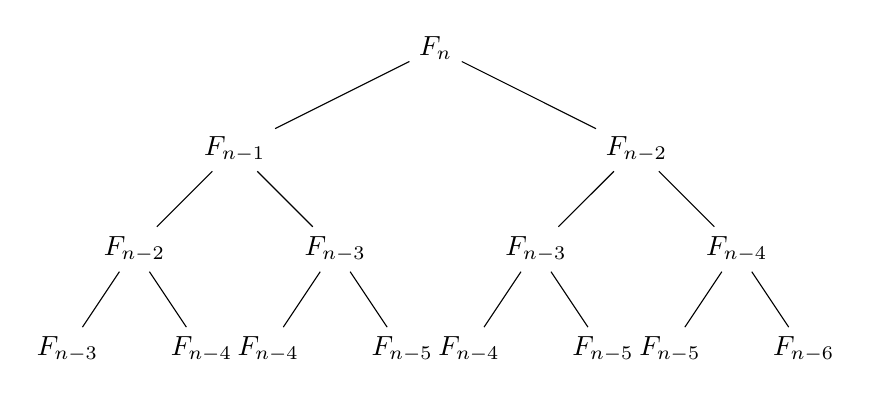
\begin{tikzpicture}[scale=0.85, level/.style={sibling distance=60mm/#1}]
\node {$F_n$}
    child {node {$F_{n-1}$}
        child {node {$F_{n-2}$}
            child {node {$F_{n-3}$}}
            child {node {$F_{n-4}$}}
        }
        child {node {$F_{n-3}$}
            child {node {$F_{n-4}$}}
            child {node {$F_{n-5}$}}
        }
    }
    child {node {$F_{n-2}$}
        child {node {$F_{n-3}$}
            child {node {$F_{n-4}$}}
            child {node {$F_{n-5}$}}
        }
        child {node {$F_{n-4}$}
            child {node {$F_{n-5}$}}
            child {node {$F_{n-6}$}}
        }
    };
\end{tikzpicture}
\caption{\texttt{fib1} 中递归调用的剧烈膨胀与重复计算}
\label{fig:fib_tree}
\end{figure}

一种更明智的方案是在中间结果——数值 $F_0, F_1, \dots, F_{n-1}$——一旦被求出时，就立刻将它们存储起来。

\begin{tcolorbox}[colback=white,colframe=gray!50!black,title={\textbf{算法}\quad \texttt{fib2}}]
\begin{algorithmic}[1]
\Function{fib2}{$n$}
    \If{$n = 0$} \Return $0$ \EndIf
    \State 创建数组 $f[0 \dots n]$
    \State $f[0] = 0,\; f[1] = 1$
    \For{$i = 2 \dots n$}
        \State $f[i] = f[i - 1] + f[i - 2]$
    \EndFor
    \State \Return $f[n]$
\EndFunction
\end{algorithmic}
\end{tcolorbox}

与 \texttt{fib1} 一样，该算法的正确性是不言自明的，因为它直接应用了 $F_n$ 的定义。它需要花费多长时间？内层循环由单步计算机操作组成，并且总共执行 $n - 1$ 次。因此 \texttt{fib2} 使用的计算机步数与 $n$ 呈\textbf{线性关系}。从指数时间骤降到多项式时间，这是运行时间上的巨大飞跃突破！现在计算 $F_{200}$ 乃至 $F_{200,000}$ 都变得轻而易举。

正如我们在全书中将反复看到的那样，\textbf{选择正确的算法将带来天壤之别}。

\subsection*{更严谨深入的分析 (More careful analysis)}

在迄今为止的讨论中，我们一直在统计每个算法所执行的基本计算机步数，并假定这些基本步花费常数时间。这是一种极其有用的简化。毕竟，处理器的指令集包含各种基础原语——分支跳转、内存存取、数字比较、简单算术等等——与其区分这些基本操作之间的细微差别，远不如将它们归为一类来得方便。

但回顾我们对斐波那契算法的处理，我们在界定何为“基本步”时显得过于随意了。如果相加的是较小的数字（比如 32 位整数），将加法视为单步计算机操作是完全合理的。但是第 $n$ 个斐波那契数大约有 $0.694n$ 个比特长，随着 $n$ 的增大，这会迅速且远远超出 32 位。对任意大的数字进行的算术运算，绝不可能在单步常数时间内完成。我们需要重新审视并修正早先的运行时间估计，使之更为真实严谨。

我们在第 1 章中将会看到，两个 $n$ 位数字相加所需的时间大约与 $n$ 成正比；如果回忆起小学一位一位处理的加法过程，这一点不难理解。因此，执行了约 $F_n$ 次加法的 \texttt{fib1}，其实际使用的基本操作步数大致与 $n F_n$ 成正比。类似地，\texttt{fib2} 所消耗的步数与 $n^2$ 成正比，这依然是关于 $n$ 的多项式，因此依然在指数级别上大幅优于 \texttt{fib1}。对运行时间分析的这一修正丝毫未曾削弱我们的突破性成果。

但是，我们能否做到比 \texttt{fib2} 还要更好？答案是肯定的：参见习题 0.4。

\section*{0.3\quad 大 O 记号 (Big-O notation)}
\addcontentsline{toc}{section}{0.3\quad 大 O 记号}

我们刚刚看到，在运行时间分析中若过于马虎草率，会导致结果出现不可接受的偏差。然而，走向另一个极端的危险同样存在：过分追求极致的精确。一次具有深刻洞察力的分析，必然建立在恰到好处的合理简化之上。

将运行时间用计算机基本步数来表达本身就已经是一种简化。毕竟，单步操作耗费的绝对时间关键取决于具体的处理器架构，甚至取决于诸如缓存策略等细枝末节（由于缓存的存在，同一段代码在不同次执行中的运行时间可能会产生微妙的差异）。考虑这些硬件层面的繁琐细节是一项如同噩梦般复杂的任务，并且其分析结论无法从一台计算机推广到另一台计算机。因此，寻求一种脱离具体机器、干净明了的算法效率刻画方式显得更有意义。为此，我们始终通过\textbf{统计基本计算机操作的步数作为输入规模的函数}来表示运行时间。

这种简化自然引出了下一步简化。我们无需报告某个算法在规模为 $n$ 的输入上需要花费诸如 $5n^3 + 4n + 3$ 步操作，省略像 $4n$ 和 $3$ 这样的低阶项要简单得多（因为随着 $n$ 的增长，它们的影响微不足道），甚至可以省略最高阶项的常数系数 5（反正几年后计算机的速度也会提升五倍），直接表述为该算法耗时 $O(n^3)$（读作“$n^3$ 的大 O”）。

现在是时候给出该记号的严格数学定义了。在下文中，我们将 $f(n)$ 和 $g(n)$ 视为两个算法在规模为 $n$ 的输入上的运行时间。

\begin{tcolorbox}[colback=white,colframe=gray!50!black]
令 $f(n)$ 和 $g(n)$ 为从正整数集到正实数集的函数。若存在常数 $c > 0$ 使得对所有 $n$ 均有 $f(n) \le c \cdot g(n)$，则我们称 $f = O(g)$（意即“$f$ 的增长速度不快于 $g$”）。
\end{tcolorbox}

说 $f = O(g)$ 是对“$f \le g$”的一种非常宽松的类比。由于常数 $c$ 的存在，它与通常的 $\le$ 概念有所不同，因此例如 $10n = O(n)$。这个常数还允许我们忽略在 $n$ 较小时发生的情况。例如，假设我们正在为某项计算任务在两种算法之间进行权衡：一种算法需要 $f_1(n) = n^2$ 步，而另一种需要 $f_2(n) = 2n + 20$ 步（图 0.2）。哪一个更好？这取决于 $n$ 的大小。当 $n \le 5$ 时，$n^2$ 更小；但在此之后，$2n + 20$ 成为绝对的胜者。在此情形下，$f_2$ 随着 $n$ 的增长具有好得多的可扩展性，因此它更为优越。

\begin{figure}[htbp]
\centering
\begin{tikzpicture}[scale=0.75]
    \draw[->] (0,0) -- (11,0) node[right] {$n$};
    \draw[->] (0,0) -- (0,11) node[above] {步数};
    \draw[domain=0:10,smooth,variable=\x,blue,thick] plot ({\x},{\x*\x/10});
    \node[right,blue] at (10,10) {$f_1(n) = n^2$};
    \draw[domain=0:10,smooth,variable=\x,red,thick] plot ({\x},{(2*\x+20)/10});
    \node[right,red] at (10,4) {$f_2(n) = 2n+20$};
    \draw[dashed] (5.24,0) -- (5.24,2.74);
    \node[below] at (5.24,0) {$n \approx 5.24$};
\end{tikzpicture}
\caption{哪种运行时间表现更好？}
\label{fig:big_o_comparison}
\end{figure}

这种优越性完全被大 O 记号所捕捉：$f_2 = O(f_1)$，因为对所有 $n$ 均有 $\frac{f_2(n)}{f_1(n)} = \frac{2n + 20}{n^2} \le 22$；另一方面，$f_1 \ne O(f_2)$，因为比值 $\frac{f_1(n)}{f_2(n)} = \frac{n^2}{2n + 20}$ 可以任意大，不存在任何常数 $c$ 能满足定义。

现在出现了第三种算法，它耗费 $f_3(n) = n + 1$ 步。它比 $f_2$ 更好吗？当然，但仅仅好在一个常数倍数因子。与 $n^2$ 和 $2n + 20$ 之间的天壤之别相比，$2n + 20$ 与 $n + 1$ 之间的差距微乎其微。为了聚焦于核心本质，如果两个函数仅相差乘法常数，我们便将它们视为等价。

回到大 O 的定义，我们看到 $f_2 = O(f_3)$（因为 $\frac{2n+20}{n+1} \le 20$），当然也有 $f_3 = O(f_2)$（取 $c = 1$）。

正如 $O(\cdot)$ 是 $\le$ 的类比，我们同样可以定义 $\ge$ 和 $=$ 的类比：
\begin{align*}
f = \Omega(g) &\iff g = O(f) \\
f = \Theta(g) &\iff f = O(g) \text{ 且 } f = \Omega(g).
\end{align*}
在前面的例子中，$f_2 = \Theta(f_3)$ 且 $f_1 = \Omega(f_3)$。

大 O 记号使我们能够专注于宏观全貌。当面对一个像 $3n^2 + 4n + 5$ 这样复杂的函数时，我们只需将其替换为 $O(f(n))$，其中 $f(n)$ 尽可能简单。在这个例子中我们使用 $O(n^2)$，因为二次项在整个和中占据绝对主导地位。以下是通过省略被支配项来简化函数的一些常识性规则：
\begin{enumerate}
    \item \textbf{乘法常数可省略}：例如 $14n^2$ 简化为 $n^2$。
    \item \textbf{若 $a > b$，则 $n^a$ 支配 $n^b$}：例如 $n^2$ 支配 $n$。
    \item \textbf{任何指数函数均支配任何多项式函数}：例如 $3^n$ 支配 $n^5$（它甚至支配 $2^n$）。
    \item \textbf{类似地，任何多项式均支配任何对数}：例如 $n$ 支配 $(\log n)^3$。这也意味着例如 $n^2$ 支配 $n \log n$。
\end{enumerate}

请不要误解对常数因子的这种淡然态度。程序员和算法设计者对常数极度重视，如果能让算法运行速度提升 2 倍，他们完全乐意通宵达旦地工作。但是在本书所处的抽象层次上，如果不借助大 O 记号所带来的简洁性，透彻理解算法的本质将是不可能的。

\newpage
\section*{习题 (Exercises)}
\addcontentsline{toc}{section}{习题}

\begin{exercise}{1}
对于下列每种情况，指出是 $f = O(g)$，还是 $f = \Omega(g)$，或两者兼成立（此时 $f = \Theta(g)$）：
\begin{center}
\begin{tabular}{lll}
& $f(n)$ & $g(n)$ \\
\hline
(a) & $n - 100$ & $n - 200$ \\
(b) & $n^{1/2}$ & $n^{2/3}$ \\
(c) & $100n + \log n$ & $n + (\log n)^2$ \\
(d) & $n \log n$ & $10n \log 10n$ \\
(e) & $\log 2n$ & $\log 3n$ \\
(f) & $10 \log n$ & $\log(n^2)$ \\
(g) & $n^{1.01}$ & $n \log_2 n$ \\
(h) & $n^2 / \log n$ & $n (\log n)^2$ \\
(i) & $n^{0.1}$ & $(\log n)^{10}$ \\
(j) & $(\log n)^{\log n}$ & $n / \log n$ \\
(k) & $\sqrt{n}$ & $(\log n)^3$ \\
(l) & $n^{1/2}$ & $5^{\log_2 n}$ \\
(m) & $n 2^n$ & $3^n$ \\
(n) & $2^n$ & $2^{n+1}$ \\
(o) & $n!$ & $2^n$ \\
(p) & $(\log n)^{\log n}$ & $2^{(\log_2 n)^2}$ \\
(q) & $\sum_{i=1}^n i^k$ & $n^{k+1}$ \\
\hline
\end{tabular}
\end{center}
\end{exercise}

\begin{exercise}{2}
证明若 $c$ 为正实数，则 $g(n) = 1 + c + c^2 + \dots + c^n$ 满足：
\begin{enumerate}
    \item[(a)] 若 $c < 1$，则 $g(n) = \Theta(1)$。
    \item[(b)] 若 $c = 1$，则 $g(n) = \Theta(n)$。
    \item[(c)] 若 $c > 1$，则 $g(n) = \Theta(c^n)$。
\end{enumerate}
\textbf{启示}：用大 $\Theta$ 语言来说，几何级数之和在严格递减时仅仅等于第一项的数量级；在严格递增时仅仅等于最后一项的数量级；而在公比为 1 保持不变时等于项数的数量级。
\end{exercise}

\begin{exercise}{3}
斐波那契数 $F_0, F_1, F_2, \dots$ 由规则 $F_0 = 0, F_1 = 1, F_n = F_{n-1} + F_{n-2}$ 定义。在本题中我们将确认该序列以指数级速度增长并求出其增长界限。
\begin{enumerate}
    \item[(a)] 使用数学归纳法证明：对所有 $n \ge 6$，均有 $F_n \ge 2^{0.5n}$。
    \item[(b)] 找到一个常数 $c < 1$ 使得对所有 $n \ge 0$ 均有 $F_n \le 2^{cn}$。证明你的答案是正确的。
    \item[(c)] 你能找到的满足 $F_n = \Omega(2^{cn})$ 的最大常数 $c$ 是多少？
\end{enumerate}
\end{exercise}

\begin{exercise}{4}
是否存在比 \texttt{fib2}（第 4 页）更快计算第 $n$ 个斐波那契数的方法？一种思路涉及矩阵。

我们首先用矩阵记号写出方程 $F_1 = F_1$ 和 $F_2 = F_0 + F_1$：
\[
\begin{pmatrix} F_1 \\ F_2 \end{pmatrix} = \begin{pmatrix} 0 & 1 \\ 1 & 1 \end{pmatrix} \begin{pmatrix} F_0 \\ F_1 \end{pmatrix}.
\]
类似地，
\[
\begin{pmatrix} F_2 \\ F_3 \end{pmatrix} = \begin{pmatrix} 0 & 1 \\ 1 & 1 \end{pmatrix} \begin{pmatrix} F_1 \\ F_2 \end{pmatrix} = \begin{pmatrix} 0 & 1 \\ 1 & 1 \end{pmatrix}^2 \begin{pmatrix} F_0 \\ F_1 \end{pmatrix},
\]
一般地有：
\[
\begin{pmatrix} F_n \\ F_{n+1} \end{pmatrix} = \begin{pmatrix} 0 & 1 \\ 1 & 1 \end{pmatrix}^n \begin{pmatrix} F_0 \\ F_1 \end{pmatrix}.
\]
因此，为了计算 $F_n$，只需将这个 $2 \times 2$ 矩阵（记作 $X$）自乘到第 $n$ 次幂。
\begin{enumerate}
    \item[(a)] 证明相乘两个 $2 \times 2$ 矩阵可以通过 4 次加法和 8 次乘法完成。
    \item[(b)] 证明计算 $X^n$ 只需要 $O(\log n)$ 次矩阵乘法。（提示：思考如何计算 $X^8$。）
\end{enumerate}
因此，我们基于矩阵的算法（称为 \texttt{fib3}）所需的算术运算次数仅为 $O(\log n)$，而 \texttt{fib2} 需要 $O(n)$。我们是否攻破了另一道指数壁垒？

问题在于我们的新算法涉及乘法，而不仅仅是加法；大数的乘法比加法要慢得多。我们已经看到，当考虑算术运算本身的复杂度时，\texttt{fib2} 的运行时间变为 $O(n^2)$。
\begin{enumerate}
    \item[(c)] 证明 \texttt{fib3} 的所有中间结果的长度均为 $O(n)$ 比特。
    \item[(d)] 令 $M(n)$ 为相乘两个 $n$ 位数算法的运行时间，并假定 $M(n) = O(n^2)$（第 1 章回顾的小学乘法能达到此界）。证明 \texttt{fib3} 的运行时间为 $O(M(n) \log n)$。
    \item[(e)] 假定对某个 $1 \le a \le 2$ 有 $M(n) = \Theta(n^a)$，你能否证明 \texttt{fib3} 的运行时间为 $O(M(n))$？（提示：被相乘的数字长度随着每次平方而翻倍。）
\end{enumerate}
结论：\texttt{fib3} 是否比 \texttt{fib2} 更快，取决于我们能否在比 $O(n^2)$ 更快的时间内完成 $n$ 位整数的乘法。你认为这可能吗？（答案在第 2 章。）

最后，斐波那契数存在解析通项公式（比奈公式）：
\[
F_n = \frac{1}{\sqrt{5}} \left( \frac{1 + \sqrt{5}}{2} \right)^n - \frac{1}{\sqrt{5}} \left( \frac{1 - \sqrt{5}}{2} \right)^n.
\]
因此看起来我们只需将几个数字提升到 $n$ 次幂就能计算出 $F_n$。问题在于这些数字是无理数，将它们计算到足够精度绝非易事。事实上，我们的矩阵方法 \texttt{fib3} 可以被看作是将这些无理数自乘到 $n$ 次幂的一种巧妙迂回途径。如果你熟悉线性代数，就应该明白为什么。（提示：矩阵 $X$ 的特征值是什么？）
\end{exercise}
